% 业余无线电通信
% 业余无线电通信.tex

\documentclass[12pt,UTF8]{ctexbook}

% 设置纸张信息。
\usepackage[a4paper,twoside]{geometry}
\geometry{
	left=25mm,
	right=25mm,
	bottom=25.4mm,
	bindingoffset=10mm
}

% 设置字体,并解决显示难检字问题。
\xeCJKsetup{AutoFallBack=true}
\setCJKmainfont{SimSun}[BoldFont=SimHei, ItalicFont=KaiTi, FallBack=SimSun-ExtB]

% 目录 chapter 级别加点(.)。
\usepackage{titletoc}
\titlecontents{chapter}[0pt]{\vspace{3mm}\bf\addvspace{2pt}\filright}{\contentspush{\thecontentslabel\hspace{0.8em}}}{}{\titlerule*[8pt]{.}\contentspage}

% 设置 part 和 chapter 标题格式。
\ctexset{
	chapter/name={第,章},
	chapter/number={\arabic{chapter}}
}

% 图片相关设置。
\usepackage{graphicx}
\graphicspath{{Images/}}

% 设置署名格式。
\newenvironment{shuming}{\hfill\zihao{4}}

% 注脚每页重新编号,避免编号过大。
\usepackage[perpage]{footmisc}

\title{\heiti\zihao{0} 业余无线电通信}
\author{童效勇(BA1AA), 陈方(BA4RC)编著}
\date{}

\begin{document}

\maketitle
\tableofcontents

\frontmatter

\begin{figure}[htbp]
	\centering
	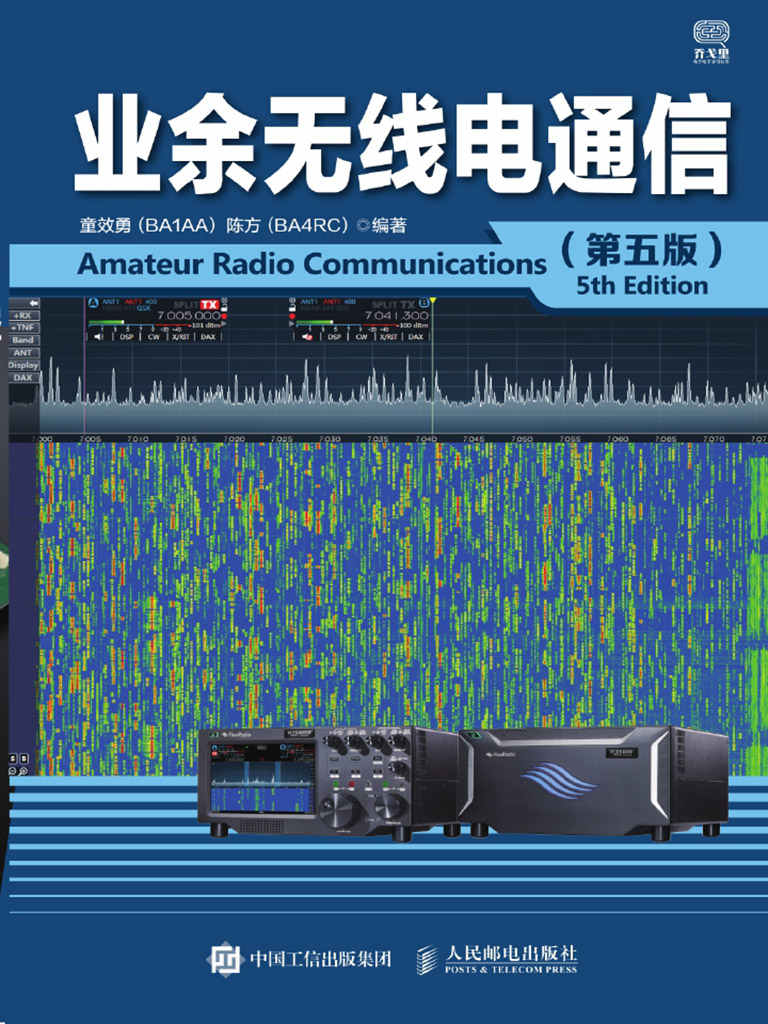
\includegraphics[width=0.7\linewidth]{cover}
	\caption{}
	\label{fig:1}
\end{figure}



\chapter{内容提要}

本书是由业余无线电家童效勇(BA1AA)和陈方(BA4RC)为广大业余无线电爱好者编写的业余无线电通信入门教材。

本书系统地介绍了开设、操作业余无线电台的相关知识和法律法规,主要内容包括:业余无线电通信简史、业余无线电通信操作实践、收发报技术的自我训练、业余无线电奖励证书和竞赛活动、不同业余无线电波段的运用、业余短波天线、业余无线电收发信机、依法设置和使用业余无线电台等。

本书既可作为开展业余无线电活动的教材,也可作为业余无线电爱好者的自修读本和手册。




\chapter{编著者的话}

业余爱好是人类社会进步的产物,是社会文明进步的标志。古今中外大凡发明创造者都有其业余爱好,而伟大的发明出自业余爱好者之手的例子更是不胜枚举。电气研究先驱者富兰克林12岁当印刷学徒并从未离开过印刷业;揭示电磁感应的法拉第也曾是报童、装订工,后来还成为一名化学专业研究者;电报机发明者莫尔斯发明电报时正从事大学的工艺美术教学……科学巨匠爱因斯坦说:“智慧并不产生于学历,而是来自对于知识的终生不懈的追求。”孔子也说:“知之者不如好之者,好之者不如乐之者。”不要被拜金主义、享乐主义和其他世俗的观点淹没了你的兴趣、爱好和激情!我们的祖国正需要千千万万个爱迪生式的发明家,而当今世界对人才的激烈竞争也正呼唤着每一个有志者从自己的业余爱好中去钻研、去实践、去塑造,以发现崭新的自我。

业余无线电通信活动以其极为丰富的内涵吸引了并将继续吸引着无数爱好者。科技性、先进性、实用性、群众性、国际性使这项活动与其他任何业余兴趣活动有着很大的不同;培养高素质的技术人才,丰富人们的文化生活,为抢险救灾提供有效的通信服务,促进各国人民间的交流,增进友谊,这一切正是改革开放不断深入的中国所迫切需要的。正因为这样,业余无线电通信活动及其标志—业余电台正越来越受到国家和各有关方面的重视,推动发展和加强管理的一系列法规、政策也已日趋完善。

我国有着大量的无线电技术爱好者,但进行业余无线电通信实践的人还不是很多。编写本书的目的是帮助更多的朋友学习和掌握业余无线电通信的基本知识和技能,尽可能地为乐于此道的爱好者们提供一本较为翔实的自我训练的教材。

改革开放的春风已吹绿了中国业余无线电通信芳草地,业余电台正如雨后春笋般出现在神州大地。愿爱好者在这里汲取更多的雨露和阳光,培育出更加绚丽夺目的奇葩—HAM之花!

1995年1月

\chapter{修订说明}

《业余无线电通信》一书自1995年出版以来,历经了数次改版、重印,2016年6月推出的第四版,也已陆续重印了三十余次。这说明在无线电技术和电子科学迅速发展的今天,这本“入门砖”性质的小册子,在广大业余无线电爱好者群体中还有一定的需求量。能够为我国业余无线电的发展尽一份微薄之力,这让我们感到十分欣慰。

为能适应科学技术和社会的快速发展以及业余无线电实践的丰富、进步,《业余无线电通信》先后于2004年、2011年和2015年进行过3次修订,出版了《业余无线电通信》第二版、第三版和第四版。在这几次修订中,除了对正文和附录里一些时效性较强的内容作必要的修改、调整外,改写了第8章《依法设置和使用业余电台》,增加了业余无线电在我国的发展简史,介绍了我国业余无线电爱好者群体在2008年汶川地震抢险救援应急通信工作中的突出表现,增加和改写了部分业余无线电通信操作实践方面的内容。

2020年10月,我们完成了《业余无线电通信》第4次修订。为能使书稿继续与时俱进,更好地服务于广大读者,我们在不改动原书总体结构的原则下,对涉及时效性的叙述及附录再次进行了修改调整,增加了软件无线电通信技术介绍、如何在线学习CW技术等方面的内容,在附录中增加了设计制作业余无线电测向机的相关内容。

《业余无线电通信》的每一次修订,都得到了许多业余无线电组织、业余无线电家和爱好者的帮助,在此一并向他们致谢。衷心感谢中国无线电运动协会,江苏、上海、天津等省、市无线电运动协会,中国无线电协会业余无线电分会以及龚万聪(BA1DU),陈平(BA1HAM),范斌(BA1RB),焦亮梅(BD1AYL),尹虎(BD1AZ),穆新宇(BD1ES),李彬(BA4REB),陈新宇(BA4RF),李家伟(BA4WI),卜宪之(BD4RG),姜锦中(BD4RQ),王龙(BD4RX),薛立人(BA5RX),郑英俊(BA5TX),陈衡(BD5RV/4),刘旭(BA8DX),刘虎(BG8AAS)等HAM在书稿校对、资料提供、翻译、新增内容的撰写等方面所给予的无私帮助,同时也感谢指正原书中的错漏之处并提出修改意见和建议的读者朋友们!

编著者

2020年10月22日

\mainmatter

无线电通信诞生于19世纪末。1888年,德国物理学家赫兹进行了一项著名的实验,他用火花隙激励一个环状天线,用另一个带缝隙的环状天线接收,证实了麦克斯韦关于电磁波存在的预言。赫兹实验激发了人们探索电磁波奥秘的热情,许多科学家都在努力研究如何利用电磁波传递信息,于是无线电技术蓬勃发展,人们的通信距离不断延伸。1901年,马可尼使用高功率的发射器首次完成了横跨大西洋的通信,揭开了无线电通信的新纪元。

20世纪初,无线电爱好者纷纷从事起无线电通信实验,商业电台数量迅速增加,电波干扰日益严重,各国政府都认识到需要制定一个法规,以保证频谱资源的合理分配和使用。1927年在华盛顿召开了世界无线电报大会,成立了国际无线电咨询委员会,并对广播、移动等各类无线电通信业务所用的频率进行了初次划分,将业余业务列入频率划分表,使业余无线电频率得到国际社会的确认。

业余无线电为无线电爱好者提供了一个广阔的舞台,无线电通信技术的发展同样也凝聚着全世界数百万业余无线电爱好者的智慧。短波通信、流星余迹通信、月面反射通信、无线电数字通信、无线电图像通信、低轨道卫星通信……业余无线电家们不断探索新的课题,在不到一百年的时间里,业余无线电从最初的无线电报逐渐发展成为利用计算机硬件、软件处理各种数字信号的全新技术。

\chapter{初识业余无线电}

从这个窗口看到的是整个世界。
——Carry V.Hammond VE3XN

1901年,马可尼成功实现了跨越大西洋的3200km距离的通信实验。1923年,业余无线电爱好者用小功率短波电台同样成功实现了横跨大西洋的通信实验。他们通过实验发现,波长越短通信距离越远,只需要较小的功率就能实现远距离通信。业余无线电爱好者的这一重大发现,是无线电发展史上最重要的成就之一,它为全球短波通信奠定了基础。

就无线电技术而言,业余无线电和其他无线电没有本质的区别。世界各国的业余无线电爱好者对无线电通信技术的发展起着重要的推动作用。在短波通信、流星余迹通信、单边带技术的研究与应用、月面反射通信、无线电数字通信、无线电图像通信、低轨道卫星通信等许多领域都留下了业余无线电家们不断探索的身影。在登山探险、抢险救灾、增进世界各国人民的友谊、培养青少年科技素质等方面,业余无线电通信也都展现了其独特的魅力和巨大潜力。

\section{独特的业余电台}

你可能很想参加业余无线电通信活动,急于了解一系列的问题,比如:

\begin{itemize}
	\item 什么是业余电台?
	\item 业余电台可以进行哪些通信实验?
	\item 业余电台能通联多远?
	\item 我能够玩转业余电台吗?
\end{itemize}  

\subsection{“火腿”与业余电台}

这里所说的“火腿”不是“金华火腿”,它特指对业余无线电通信有着浓厚兴趣的人。业余无线电爱好者的英文是“Radio Amateur”,又称为“HAM”。由于“HAM”在英语中还可以被解释为“火腿”(见图1-1),所以“火腿”又成了业余无线电通信爱好者们的另一个名字。

\begin{figure}[htbp]
	\centering
	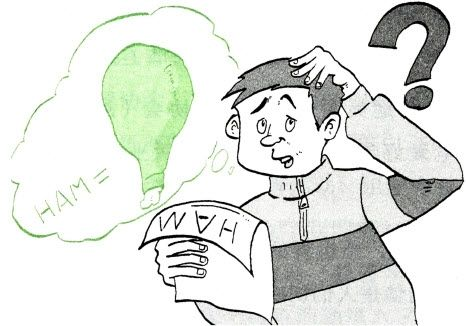
\includegraphics[width=0.7\linewidth]{1}
	\caption{业余无线电通信爱好者}
	\label{fig:1}
\end{figure}

业余无线电台(Amateur Radio Station)是经过国家无线电主管部门正式批准,业余无线电爱好者为了试验收发信设备,进行技术探讨、通信训练和比赛而设立的电台。业余电台中的“业余”一词,并不表示从事业余无线电通信活动的人缺少专业知识与技能,而是强调业余无线电不能用于商业目的。国际电信联盟(ITU)根据不同的用途将全世界所有无线电通信分为43种业务,业余电台属于其中的“业余业务”。ITU对业余业务的定义为“供业余无线电爱好者进行自我训练、相互通信和技术研究的无线电通信业务。业余无线电爱好者系指经正式批准的、对无线电技术有兴趣的人,其兴趣纯系个人爱好而不涉及谋取利润”。

世界各国政府对业余无线电活动都给予了多方面的支持,允许无线电爱好者通过无线电波跨越国界进行国际间的交流,因此业余无线电爱好者也被称为各国的民间友谊大使。目前全世界拥有电台呼号的爱好者约300万人,如果你拥有了自己的电台和呼号,成为“火腿族”的一员,你就可以和国内外的业余无线电爱好者进行空中对话了。

下面摘录的是美国业余无线电协会(ARRL)出版的《业余无线电爱好者手册》中一段有关业余无线电通信的说明。

“一年365天,全世界的业余无线电爱好者都随时相互进行着通信。通信是人们切磋有趣的技术,进行富于变化的、激动人心的试验,发现新朋友的手段。业余无线电家作为具有共同的广泛兴趣的人们,通过全球规模的‘友谊之桥’,进行空中通信,交换思考的话题,互相学习。因此,业余无线电通信具有超越国界、增强理解和友谊的作用。这一点是其他爱好所无法实现的”。

\subsection{集体电台和个人电台}

根据设台者的身份,业余电台分为集体电台和个人电台两种。由团体申请设置,并由设台团体使用的称为集体业余电台,国际上常称其为俱乐部台(Club Station)。我国现有的集体业余电台,多为体育、教育、科协等系统所设立,是组织、培训爱好者的活动中心。个人业余电台是指爱好者本人申请设置并由其本人操作使用的电台。当今世界300万个业余电台中,绝大多数是个人电台。

中国的业余无线电活动开始于20世纪20年代,在当时极其简陋的条件下,老一辈业余无线电家怀着“以科学报效祖国”的理想,自己动手制作无线电收、发报机,互相联络,成为掌握无线电通信技术的先锋。新中国成立后,党和国家领导人十分重视在青少年中开展无线电活动,参照前苏联建立“陆海空志愿协会”军事后备组织的模式,我国建立了中国人民无线电俱乐部等机构,陆续从东欧引进快速收/发报、无线电测向、无线电多项通信等活动,组建专业运动队参加国际比赛。1958年在北京建立了我国第一座集体业余电台BY1PK。1992年,经国务院批准,我国恢复开放个人业余电台。从此,我国的业余无线电活动进入了一个新的阶段。近年来,随着中国经济的飞速发展和世界范围内文化交流的加强,业余无线电已揭开它神秘的面纱,逐步成为许多爱好者业余生活的重要内容,如图1-2所示。各地的业余无线电爱好者积极加入到普及通信知识和操作技能的活动中,时刻准备在突发灾害到来时为社会服务。还有的爱好者正在进行数据通信、空间通信等各种新技术的研究。

\begin{figure}[htbp]
	\centering
	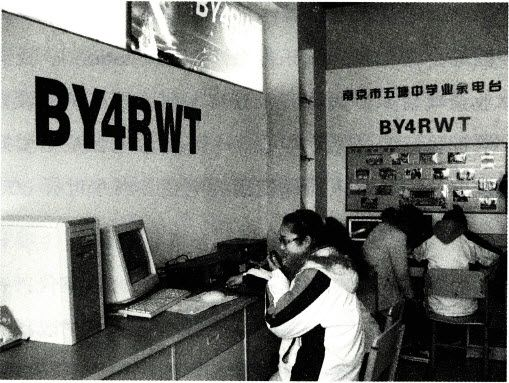
\includegraphics[width=0.7\linewidth]{2}
	\caption{业余电台BY4RWT}
	\label{fig:1}
\end{figure}

\section{业余无线电活动}

业余无线电爱好者进行通信实验的内容是极其丰富的,既有“古老”的电报通信,也有各种各样的数据通信和图像通信。世界各国的爱好者还把电台设备带到野外相互通联,进行移动通信、小功率通信实验。捕捉“突发E层”、“大气波导”进行VHF/UHF波段超远程通信试验是最具魅力的研究课题之一,将互联网与电台结合在一起的Ecohlink同样也吸引着众多的业余无线电爱好者。

\subsection{数字通信}
数字通信是指传递数字信号的通信模式。通信的数字化,是当今通信技术的发展趋势之一。业余通信中的数字通信模式可以说是层出不穷,直到今天还在业余界广泛使用的电报(CW)应该算是最古老的一种数字通信模式。无线电电传(RTTY)是一种对设备要求较低的数字通信模式,在发送端用键盘代替话筒或电键输入信息,接收端则把来自对方的文字显示在显示器上,如图1-3所示。AMTOR是一种具有纠错码功能的电传通信方式。这种通信方式把每一个信息分散在不同时间里重复发送,在不增加设备的情况下,可以大大改善通信系统的可靠性。

\begin{figure}[htbp]
	\centering
	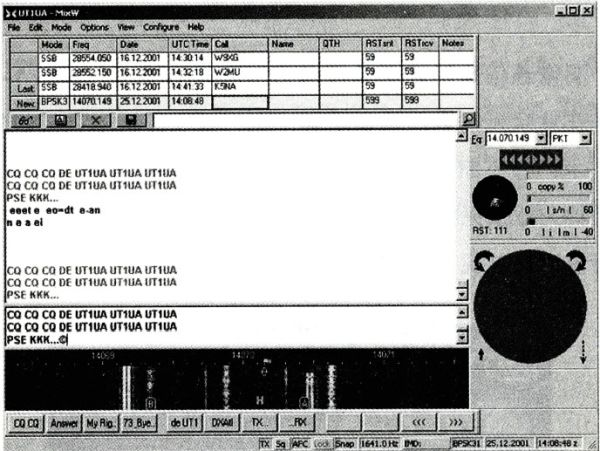
\includegraphics[width=0.7\linewidth]{3}
	\caption{数字通信软件}
	\label{fig:1}
\end{figure}

PSK31是指带宽为31Hz的移相键控调制模式。它只需要31Hz的带宽,占用频带非常窄,抗噪声能力强。当非常微弱甚至是几乎不可闻的信号出现时,只要在计算机屏幕上能出现信号轨迹,一般都能正确地解调。

另一种被广泛使用的数字通信模式是PACKET,利用广泛存在的PACKET网络,业余爱好者们每时每刻都能传递各种各样的信息,美国的爱好者甚至还利用PACKET网络提供全国范围的业余定位系统服务。

除此之外还有PACTOR、CLOVER、G-TOR等其他的数字通信模式,每种不同的模式适合不同的应用场合,各有各的特点。各种模式的通信实验给热衷于数字通信的业余无线电爱好者带来了许多乐趣。

\subsection{图像通信}

图像通信是现代通信技术综合发展的结果,如图1-4所示。在业余无线电通信领域里,也一直在探讨电视图像的传送技术,并不断对其进行改进。图像通信有两种主要方式;一种称为业余无线电视(ATV),用于传送活动图像;另一种称为慢扫描电视(SSTV),用于传送静止图像。

\begin{figure}[htbp]
	\centering
	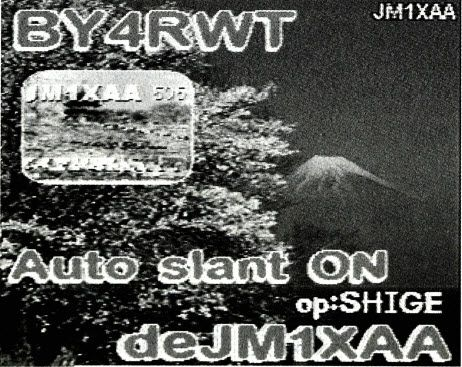
\includegraphics[width=0.7\linewidth]{4}
	\caption{图像通信}
	\label{fig:1}
\end{figure}

普通电视为保证图像清晰,每秒需传送50幅图像,要占用6MHz宽的频带。业余频段范围较窄,难以传送一般的电视信号。爱好者采用几秒传送一幅图像的办法,用图像信号的慢变化来减小频带宽度,使得在短波波段传送图像的愿望得以实现。现在,许多爱好者借助计算机技术,配合简单的接口电路及软件,就可以完成SSTV方式的通联,这极大地丰富了业余无线电通信的内容。

\subsection{业余卫星通信}

1957年10月4日前苏联发射了世界上第一颗人造地球卫星,与此同时,美国的一些爱好者萌发了发射业余通信卫星的设想。他们组织起来并将这个计划命名为OSCAR。4年之后,他们的努力获得成功,世界上第一颗业余通信卫星OSCAR-1号在美国加利福尼亚的范登伯格空军基地发射升空。这不但证明了业余无线电爱好者有能力研制、开发、控制自己的卫星,也标志着业余无线电通信从此进入了太空时代。

业余卫星通信系统分为空间部分和地面部分。空间部分是指业余通信卫星,地面部分就是我们的业余电台。一个业余卫星地面电台由收发信设备、天线和跟踪控制系统组成。

在卫星通信中,由于通信距离远,信号传输损耗较大,卫星通信天线需要有较高的增益。VHF/UHF频段多采用8~10单元的八木天线,更高的频段使用20单元的八木天线或是抛物面天线。由于低轨道卫星运行周期较短,天线系统还应具备自动跟踪的功能。一般把发送、接收天线集中安装在可沿水平轴和垂直轴旋转的云台上,根据室内提供的驱动信号完成跟踪。

业余卫星通信爱好者可以选用专用的卫星收、发信机,能够异频双工工作。如YAESU公司的FT-736就是一种VHF/UHF频段全模式的卫星收、发信机,能在50MHz、144MHz、220MHz、430MHz和1200MHz业余波段工作,有SSB、CW和FM模式,能够同时异频收、发。这对于在低轨道卫星通信中克服多普勒频移很有作用。

低轨道卫星的特点是运行速度快,一般每两小时绕地球一周。要与低轨道卫星通信,必须能精确地确定卫星的位置。现在已有专门的软件可以计算出业余卫星的轨道,可以知道卫星什么时候经过我们的上空,算出卫星的仰角和方位角,由计算机控制天线方向控制器,使天线始终指向卫星,自动完成对卫星的跟踪,如图1-5所示。由于天线的波束宽度有一定的范围,也可通过手动方式控制天线方向。

\begin{figure}[htbp]
	\centering
	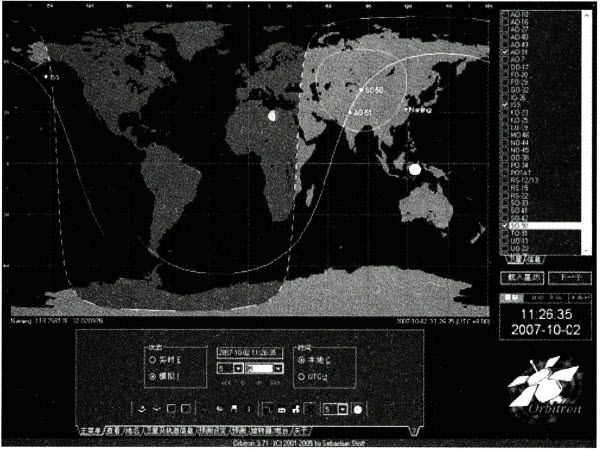
\includegraphics[width=0.7\linewidth]{5}
	\caption{卫星跟踪软件}
	\label{fig:1}
\end{figure}

世界各国的业余无线电爱好者已经成功地发射了二十几颗业余卫星。2009年12月15日,“希望一号”卫星(HO-68,见图1-6)在太原卫星发射中心搭载“长征四号丙”运载火箭成功地进入太空,见图1-7。这是中国第一颗青少年科普卫星。广大的业余无线电爱好者可以通过“希望一号”卫星进行各种方式的通信实验。

\begin{figure}[htbp]
	\centering
	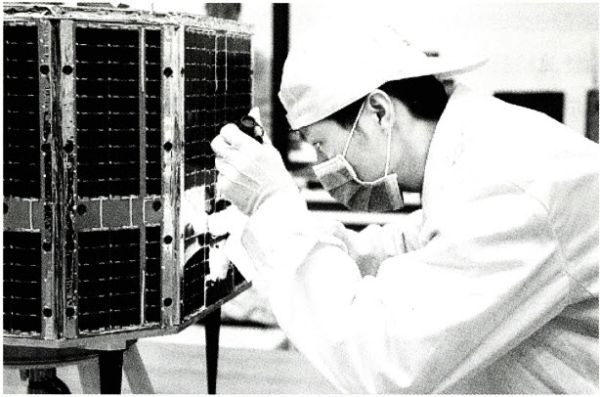
\includegraphics[width=0.7\linewidth]{6}
	\caption{技术人员在测试“希望一号”卫星}
	\label{fig:1}
\end{figure}

\begin{figure}[htbp]
	\centering
	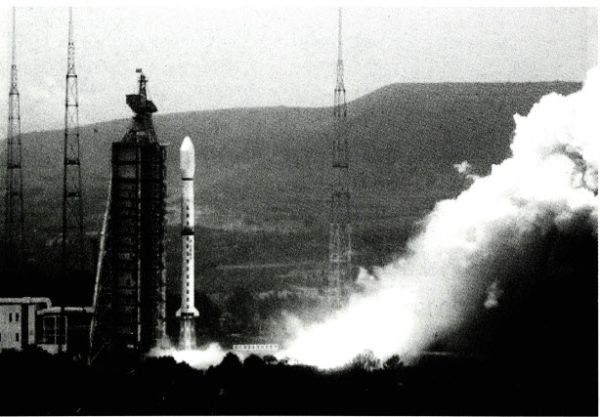
\includegraphics[width=0.7\linewidth]{7}
	\caption{“希望一号”卫星搭载“长征四号丙”运载火箭成功进入太空}
	\label{fig:1}
\end{figure}

\subsection{国际空间站业余无线电通信计划}

和国际空间站宇航员对话是一种独特的体验。国际空间站业余无线电通信计划(ARISS)是由美国业余无线电协会、国际业余卫星公司、美国国家宇航局等共同组织和发起的一项活动,是美国国家宇航局面向青少年的科技教育项目之一,图1-8所示为美国等16个国家共同建造的国际空间站。这个计划给学生们提供了一个利用业余无线电和国际空间站宇航员直接交流的机会。该计划要求学生用英语提出有关太空、太空飞行、宇航员的太空生活等的问题,宇航员对学生提出的问题进行解答。因此要求学生有较好的英语口语和听力水平,同时对太空知识有一定的了解。从2000年到2010年,世界上大约有400所学校参与了这项活动。

\begin{figure}[htbp]
	\centering
	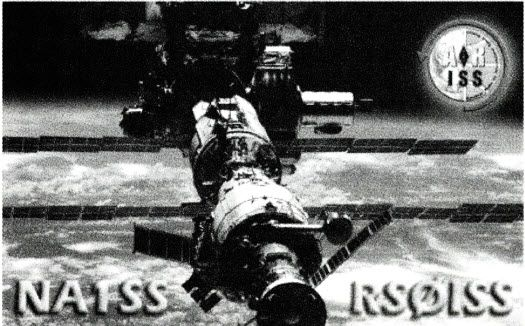
\includegraphics[width=0.7\linewidth]{8}
	\caption{国际空间站}
	\label{fig:1}
\end{figure}

“Can you see the Great Wall from the ISS?”2007年8月26日北京时间18:44,南京市第三中学初二学生唐洁雯用流利的英语向宇航员提出了第一个问题,克莱顿·安德森在距地球300km的国际空间站上听到来自中国学生的呼叫。经过两年的不懈努力和等待之后,BY4RRR与国际空间站的通联活动终于得以实现。图1-9所示是中国学生第一次通过ARISS的国际计划,直接与国际空间站上的宇航员对话的情景。

\begin{figure}[htbp]
	\centering
	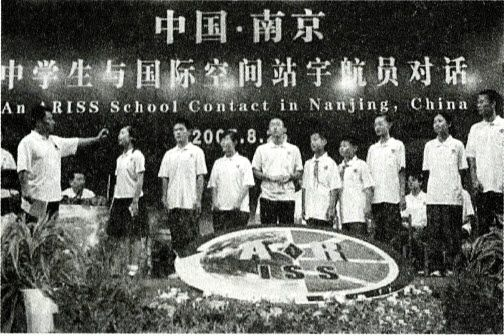
\includegraphics[width=0.7\linewidth]{9}
	\caption{BY4RRR的同学与国际空间站宇航员对话}
	\label{fig:1}
\end{figure}

\subsection{月面反射通信}

依靠月面反射完成通联的这种通信方式称为EME(Earth Moon Earth),见图1-10。地球与月球之间的距离大约为380000km,电波往返一次衰减极大,月面反射通信返回到地面的信号非常微弱。要想完成一次EME联络,必须掌握无线电波的传播特点,知道月亮的阴晴圆缺产生的不同的天体噪声对接收的影响。进行EME通信必须配备大功率发射机、高增益天线(见图1-11)以及高灵敏度的接收机。目前,完成双向EME联络大多数为CW方式。

\begin{figure}[htbp]
	\centering
	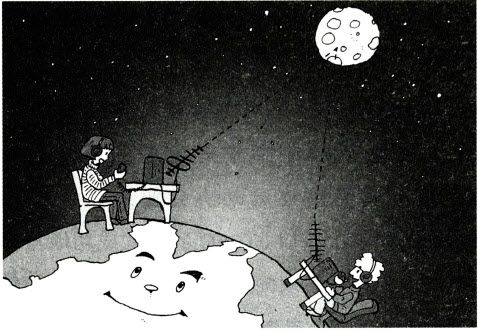
\includegraphics[width=0.7\linewidth]{10}
	\caption{月面反射通信}
	\label{fig:1}
\end{figure}

\begin{figure}[htbp]
	\centering
	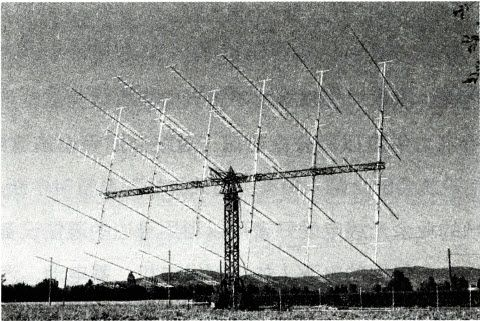
\includegraphics[width=0.7\linewidth]{11}
	\caption{用于月面反射通信试验的八木天线阵}
	\label{fig:1}
\end{figure}

20世纪40年代,业余无线电家们已向EME通信发起了挑战。经过许多次失败之后,终于在1960年,美国的W6HB和W1BU在1296MHz首次实现了EME通信。

我国业余无线电爱好者也在积极探索EME通信。1997年10月19日,清华大学业余电台BY1QH在2m波段和瑞典SM5FRH等业余电台成功地进行了双向的EME联络,实现了我国在这一领域零的突破。

现在,EME通信已采用由计算机完成的新的调制技术,这大大降低了EME通信对设备的要求。2007年5月20日,江苏省无线电运动协会业余电台BY4RSA在1296.090MHz频率上,以JT65C的模式成功地与荷兰的业余电台PA3CSG进行了双向EME通联。这次实验使用的是一台IC706电台,一个自制的变频器和直径为1.8m、增益为25dB的抛物面天线,一台自制的功率放大器,发射功率仅90W。

\subsection{应急通信}

当地震、洪水、恐怖袭击等重大灾害事故突然发生时,往往伴随着电力供应以及公众电信、道路交通等设施遭到破坏,常规通信设施会随之陷入瘫痪,与外界的联系暂时中断。这时,灾害现场的业余无线电爱好者可以利用身边的通信设备,尽快找到可供电台使用的电源(如小型发电机、蓄电池、汽车电源等),选择有利地形,迅速架设天线,并立即进行紧急“求救呼叫”。在美国“9·11”恐怖袭击事件、印尼大海啸、四川汶川地震等灾难中,业余无线电爱好者在应急通信中都发挥了重要的作用。

在VHF/UHF频段,可用语言直接进行求救呼叫。

例如:“May Day、May Day、May Day! BA4AAA求救,BA4AAA求救,听到请回答。”

在求救呼叫得到灾害现场以外地区的回答后,呼救电台应向外发送以下信息:

①受灾的精确地点及性质(即遭受何种灾害);

②受灾的程度及受灾现场的情况;

③灾害现场现有的救援力量及迫切需要何种支援。

④其他一切有利于援助的资料。

求救呼叫是最高级别的信号,任何业余电台收听到求救呼叫时,必须立即无条件中断发射,改为守听状态,并给予必要的协助。

呼救电台在紧急情况得到解决后,应及时在结束联络时清楚地发出解除呼救的信号,以免其他电台继续长时间守听。
例如:“我是BA4AAA,救援人员已经到达,BA4AAA解除呼救,BA4AAA解除呼救,再见。”

承担救灾应急通信是业余电台的社会责任和优良传统,也是业余频段得到保护的主要理由之一。世界上许多国家都成立了业余无线电应急服务组织,美国ARRL有专业的业余无线电通信应急服务(ARES)委员会,我国的无线电爱好者也在积极开展应急通信演练活动(见图1-12),筹划、建立各地区的业余无线电应急通信网络。

\begin{figure}[htbp]
	\centering
	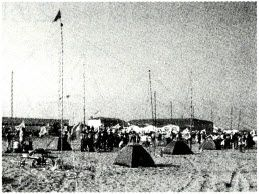
\includegraphics[width=0.7\linewidth]{12}
	\caption{应急通信演练}
	\label{fig:1}
\end{figure}

\section{依法设置业余电台}

为了有效利用无线电频率资源,保证各种无线电业务的正常进行,国际电信联盟制定了无线电管理的国际法规——《无线电规则》,用来作为各国无线电管理的依据。1993年国务院、中央军委颁布了《中华人民共和国无线电管理条例》,国家无线电管理机构先后颁布了一系列规章和管理文件。这些规定是我们开展业余无线电活动必须遵循的准则。
业余无线电爱好者不同于一般的电子技术爱好者,设置和使用个人业余电台,进行无线电波的发射,必须向国家或者地方无线电管理机构提出申请,得到批准并取得《中华人民共和国无线电台执照》(以下简称《电台执照》),严格按照指配的频率、功率工作。未经批准擅自使用无线电通信设备,干扰其他无线电通信业务的正常工作,造成空中电波秩序混乱,违规者将受到警告、查封及没收设备、罚款、吊销《电台执照》等处罚。造成严重后果、构成犯罪的,将依法追究刑事责任。

\subsection{取得业余电台《操作证书》}

根据国家无线电管理机构的有关规定,设置个人业余电台必须持有《中华人民共和国业余无线电台操作证书》(以下简称《操作证书》),如图1-13所示。《操作证书》是设置操作业余电台所要求的技术凭证。它共分5个等级,一级为最高级,五级为收听级。

\begin{figure}[htbp]
	\centering
	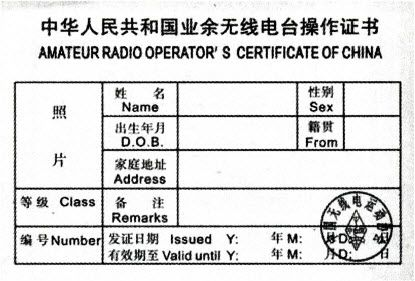
\includegraphics[width=0.7\linewidth]{13}
	\caption{《中华人民共和国业余无线电台操作证书》}
	\label{fig:1}
\end{figure}

申请《操作证书》者,应是经过无线电管理机构委托的中国无线电运动协会或其他单位的培训,并经《操作证书》考核机构考试合格的中华人民共和国公民。申领《操作证书》没有年龄限制。

取得《操作证书》后,可凭证在国内的个人和集体业余电台上进行操作,但必须得到电台的设台人或负责人同意,使用所操作电台的呼号,并严格遵守该台及《电台执照》中的各项规定。操作时使用的功率、频率及操作方式不得超越本人《操作证书》允许的范围。

取得《操作证书》后,如果打算设置个人业余电台,可按当地无线电管理机构规定的渠道递交《设置个人业余电台申请表》,并按当地无线电管理机构的要求对电台设备进行检验、检测,批准并核发《电台执照》,如图1-14所示,同时指配业余电台呼号。只有获得《电台执照》后,爱好者才能使用分配给自己的呼号,按照规定与国内外业余电台进行联络和交换QSL卡片。

\begin{figure}[htbp]
	\centering
	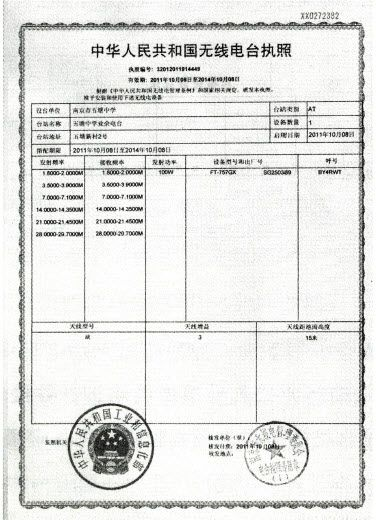
\includegraphics[width=0.7\linewidth]{14}
	\caption{《中华人民共和国无线电台执照》}
	\label{fig:1}
\end{figure}

\subsection{设置业余电台}

需要注意的是,部分初学者不了解有关的法规,购买到对讲机等通信设备后,自行设置频率,无证(照)发射。或虽有《操作证书》和《电台执照》,但使用时随意改变《操作证书》所允许的频率、功率范围,干扰其他电台,这都是与有关法规相违背的。

\subsection{工业和信息化部无线电管理局}
工业和信息化部无线电管理局是国家无线电管理机构,负责无线电频率的划分、分配与指配;依法监督管理无线电台(站);负责卫星轨道位置协调和管理;协调处理军地间无线电管理相关事宜;依法组织实施无线电管制;负责无线电监测、检测、干扰查处,协调处理电磁干扰事宜,维护空中电波的秩序。国家无线电管理机构和地方无线电管理机构负责业余电台的管理工作。

4.中国无线电运动协会
中国无线电运动协会(CRSA,见图1-15)是全国无线电爱好者的群众性组织,是主管业余无线电活动的政府部门联系广大无线电爱好者的纽带和管理业余无线电活动的助手。中国无线电运动协会在国际业余无线电联盟(IARU)中代表中国业余无线电爱好者。

\begin{figure}[htbp]
	\centering
	
\includegraphics[width=0.7\linewidth]{15}
	\caption{CRSA会徽}
	\label{fig:1}
\end{figure}

目前,不同省、自治区、直辖市的业余无线电爱好者加入中国无线电运动协会,参加业余电台操作培训和考核,申请设置使用业余电台所需履行的具体手续有所不同,可向当地无线电管理机构、中国无线电运动协会或地方业余无线电社团咨询。中国无线电运动协会的总部设在北京,通信地址为“北京6106信箱”,邮政编码:100061,网址www.crsa.org.cn。

\subsection{国际电信联盟}

国际电信联盟是联合国的一个专门机构,也是联合国机构中历史最长的一个国际组织,简称“国际电联”、“电联”或“ITU”。国际电联是主管信息通信技术事务的联合国机构,主要负责各种业务间的频率分配。国际电联总部设在瑞士日内瓦,其成员包括191个成员国和700多个部门成员。

\chapter{选购一部业余电台}

引子
最好的选择未必是选择最好的。

可供爱好者选择的业余电台品种很多。按照不同的分类方法,可将业余电台分为单波段电台、双波段电台、多波段电台,或是手持式电台、车载电台、短波电台和全波段电台。尽管各种电台的外形、大小不尽相同,每部电台都由一些基本组件构成,它们是:电源、发射/接收机和天线,如图2-1所示。

\begin{figure}[htbp]
	\centering
	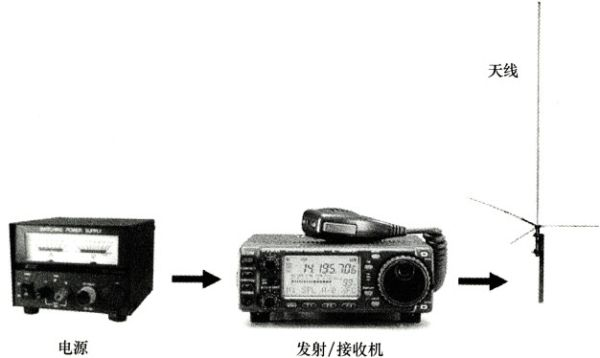
\includegraphics[width=0.7\linewidth]{16}
	\caption{电源、发射/接收机和天线是业余电台的3个基本组件}
	\label{fig:1}
\end{figure}

业余电台是指可以工作在业余频段的电台设备。购买电台之前,先要知道与电台设备密切相关的一些知识,如频率、频段、调频、调幅、功率等,以便在选购时对电台的特点有一个初步的了解。购买电台需要考虑许多因素,首先要确定电台的类型,然后再根据通信距离和通信环境来选择工作频段及输出功率。电台又是一种特殊的商品,购买、使用时还必须了解有关的法规和政策。

\section{业余频段}

人们可利用的电磁波的频率从千分之几赫直至1030Hz。为了便于研究、使用和管理,国际上把整个无线电频谱划分为若干频带,通常称为频段或波段。无线电波频段的划分见表2-1。电磁波是人类共享的资源,为了合理使用这一资源,国际电信联盟(ITU)对广播、移动等各种无线电业务可以使用的频率作了规定和划分。业余无线电通信作为业余业务在各频段上也都占有一席之地。这就是供全世界业余无线电爱好者使用的业余频段,我国业余电台使用的频率以《中华人民共和国无线电频率划分规定》为依据,表2-2列出的是常用的业余频段名称和频率范围。

\begin{figure}[htbp]
	\centering
	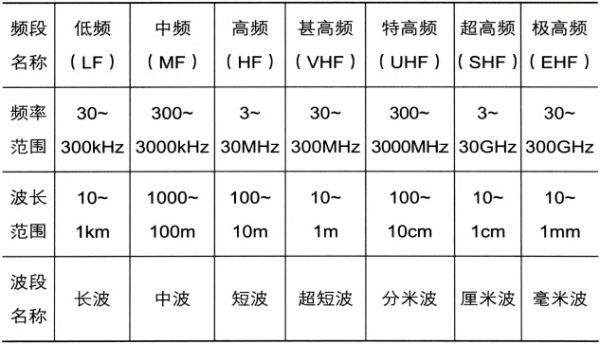
\includegraphics[width=0.7\linewidth]{17}
	\caption{无线电波频段的划分}
	\label{fig:1}
\end{figure}

\begin{figure}[htbp]
	\centering
	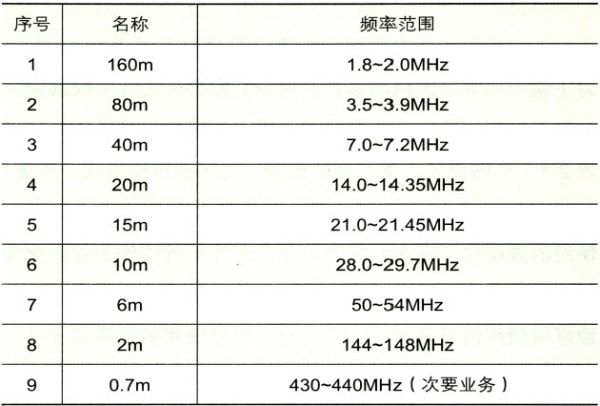
\includegraphics[width=0.7\linewidth]{18}
	\caption{业余业务频段}
	\label{fig:1}
\end{figure}

\section{VHF/UHF手持业余电台}

手持业余电台又称为对讲机,它是一种小型的移动通信工具,如图2-2所示。手持业余电台的最大优点是携带方便,野外活动时可以将手持业余电台抓在手上或放入衣袋中,手持业余电台主要用于FM通信。

VHF(甚高频)是指频率从30~300MHz的无线电波,UHF(特高频)是指频率从300~3000MHz的无线电波。实际上某个VHF/UHF手持业余电台的工作频率范围只是甚高频或特高频整个频段的一部分。

手持业余电台多为VHF/UHF单频段电台,也有许多手持业余电台可以多频段通信。例如八重洲VX-7R手持业余电台可以在50MHz、144MHz、430MHz 3个业余频段上通信。

由于受到体积的限制,手持业余电台不能提供较大的输出功率,手持业余电台所配的橡胶天线效率很低(见图2-3),这些因素使得手持业余电台的通信距离很有限,开阔地的通话距离为几千米。

\begin{figure}[htbp]
	\centering
	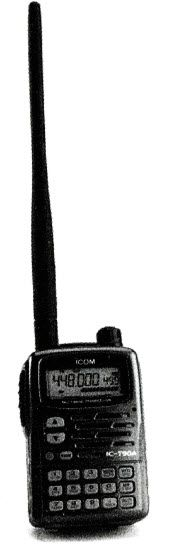
\includegraphics[width=0.7\linewidth]{19}
	\caption{FM手持业余电台}
	\label{fig:1}
\end{figure}

\begin{figure}[htbp]
	\centering
	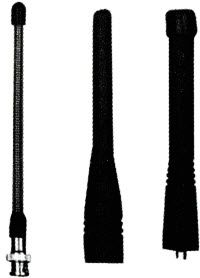
\includegraphics[width=0.7\linewidth]{20}
	\caption{螺旋橡胶天线}
	\label{fig:1}
\end{figure}

VHF/UHF波段手持业余电台设备的价格低廉,可选范围大。VHF/UHF波段又是爱好者的“入门波段”,世界上大多数爱好者都活跃在这个波段上。

\section{VHF/UHF车载业余电台}

车载业余电台是专门为汽车和其他交通工具设计制造的移动通信设备,车载业余电台仅能在业余频段发射信号。车载业余电台设计紧凑,外壳坚固结实,结构耐冲击和震动。电台大小一般按汽车收放机的大小标准设计,主操作通过前面板进行,较先进的机型还采用分离式面板的安装形式,方便在车内狭小的空间内安装。图2-4所示为一部八重洲双段车载业余电台。车载业余电台为我们带来驾驶车辆以外的另一种感受,利用车里的业余无线电设备进行通联,可以体验野外通信的乐趣。图2-5所示为一部车载业余电台在车内的安装位置。

\begin{figure}[htbp]
	\centering
	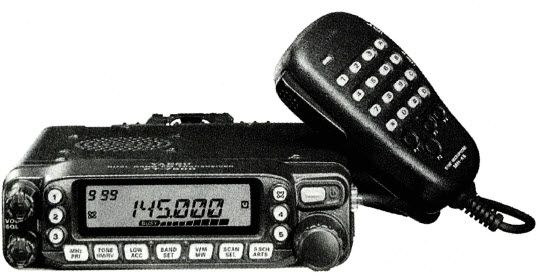
\includegraphics[width=0.7\linewidth]{21}
	\caption{八重洲FT-7800R VHF/UHF双段车载业余电台}
	\label{fig:1}
\end{figure}

\begin{figure}[htbp]
	\centering
	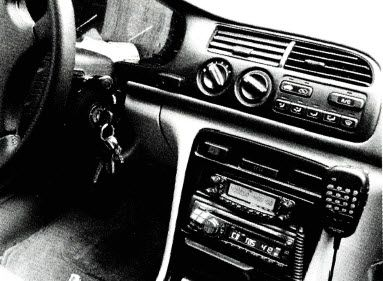
\includegraphics[width=0.7\linewidth]{22}
	\caption{车载业余电台安装的位置}
	\label{fig:1}
\end{figure}

车载业余电台具有较大的输出功率。在进行FM通信时,大功率能够通联更远的距离。但是,业余电台选用设备的最大输出功率不得超过无线电管理部门核发的《电台执照》所规定的功率。当然,车载业余电台也可以放在室内使用,接上电源和室外天线,它就是一部基地电台了。

在移动通信中,由于电台位置不断变化,为保证通信质量,一般要求移动电台及基地台天线在水平面内无方向性,并且采用垂直极化方式。我们通常看到工作在VHF/UHF频段的手持业余电台、车载业余电台、中继台都使用了各种形式的垂直极化无指向性天线。

车载天线(见图2-6)有吸盘天线和夹边天线两种。车载天线在结构上有1/4波长天线、1/2波长天线、5/8波长天线等形式。一般情况下天线越长,其增益也越高。若通信范围主要是在市区通过中继台进行通联,则可以选择增益较低的短天线。当用于郊外车辆间远距离联络时,宜选用高增益的长天线。由于高度的限制,加上车辆高速行驶时会遇到很大的风阻,所以车载天线的尺寸要依照工作频段采用不同的设计。

\begin{figure}[htbp]
	\centering
	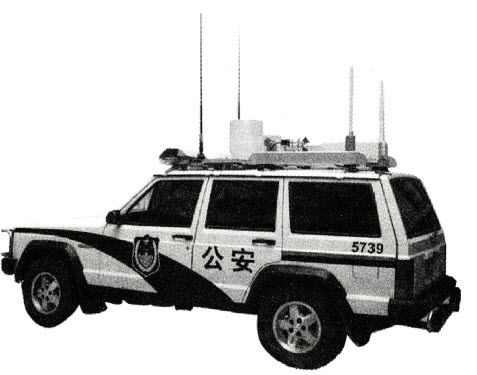
\includegraphics[width=0.7\linewidth]{23}
	\caption{车载天线}
	\label{fig:1}
\end{figure}

车载天线大多数是VHF/UHF双频段天线,这样只要一根天线就可以同时进行VHF频段和UHF频段的发射和接收。一般车载天线都是采用垂直极化方式,这种天线在水平方向上是均匀辐射的,这可以让我们在驾驶中不需要时刻想着天线的方向。图2-7所示是平面接地(GP)天线的立体方向图,这是一种典型的垂直极化全向天线。

\begin{figure}[htbp]
	\centering
	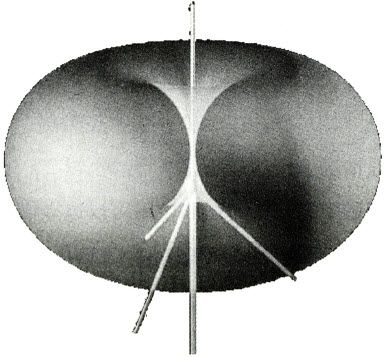
\includegraphics[width=0.7\linewidth]{24}
	\caption{GP天线方向图类似苹果形状}
	\label{fig:1}
\end{figure}

\section{短波业余电台}

短波(HF)业余电台是指发射频率在1.5~30MHz之间各业余频段的电台设备。图2-8所示为一部IC-718短波业余电台。短波业余电台的优点之一就是不需要很大的发射功率就能实现远距离通信。短波业余电台的输出功率通常为100W,在传播条件良好的情况下,这个功率可以进行全球范围的通信。

\begin{figure}[htbp]
	\centering
	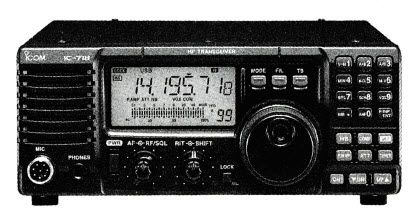
\includegraphics[width=0.7\linewidth]{25}
	\caption{ICOM IC-718短波业余电台}
	\label{fig:1}
\end{figure}

短波波段是比较常用的业余无线电波段,在这个波段上,业余无线电爱好者可以使用多种通信模式,其中包括:

\begin{itemize}
	\item SSB—单边带语音模式;
	\item CW—电报模式;
	\item AM—调幅语音模式;
	\item FM—调频语音模式;
	\item RTTY—无线电电传模式;
	\item SSTV—慢扫描电视模式。
\end{itemize}

目前,有些制造厂商设计出了HF/VHF/UHF多波段、多模式业余电台,发射频率范围可达1.9~440MHz间的各业余频率。我们将这类电台称作全波段电台,它是目前非常流行、畅销的电台,如图2-9所示。全波段电台既可以作为移动台,也可以作为基地台。一些全波段电台还具有业余卫星通信等扩展功能。

\begin{figure}[htbp]
	\centering
	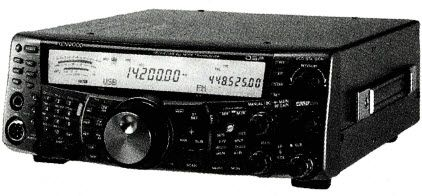
\includegraphics[width=0.7\linewidth]{26}
	\caption{建伍TS-2000 1.8~440MHz全波段电台}
	\label{fig:1}
\end{figure}

天线是无线电通信设备的耳目,天线的质量直接影响着电台通联的效果。电台通过天线向空中发射无线电波,同时通过天线从空中接收无线电信号,因此对电台来说,天线具有特别重要的作用。每部电台必须配备性能良好的天线才能实现好的通联效果。

短波业余电台常用的天线有半波偶极天线和八木天线。半波偶极天线是最容易制作的天线。它的结构非常简单,只需要将两根长度相同、总长度约为半波长的导线水平架设起来即可。偶极天线的长度由工作频率决定。以7MHz频段为例,它的波长λ≈42.85m。业余无线电爱好者通常将这个数字简称为40m,因此7MHz频段也称作40m波段。半波偶极天线两段导线的长度是1/4λ=10.7m,其外形如图2-10所示。

\begin{figure}[htbp]
	\centering
	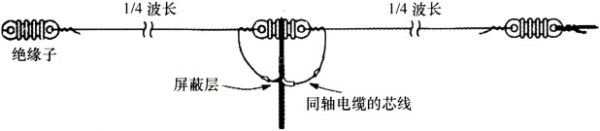
\includegraphics[width=0.7\linewidth]{27}
	\caption{水平半波偶极天线}
	\label{fig:1}
\end{figure}

八木天线是一种典型的定向天线。这种天线是由日本人八木秀次于1926年发明的,因此叫做八木天线。八木天线具有良好的方向性和高增益,配合转向器可以很好地工作在HF、VHF和UHF频段,图2-11所示为一个典型的短波八木天线。将多个八木天线组合起来,构成天线阵列,可以进一步提高八木天线的方向性,特别适合VHF/UHF频段远距离通联。

\begin{figure}[htbp]
	\centering
	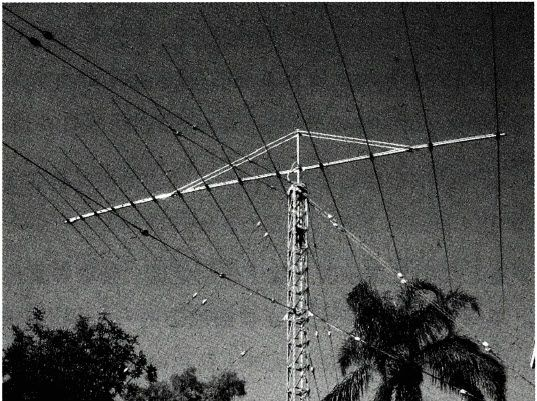
\includegraphics[width=0.7\linewidth]{28}
	\caption{HF频段14单元八木天线}
	\label{fig:1}
\end{figure}

\section{几个常用术语}

\subsection{频率范围}
为了合理地利用频率资源,保证用户之间不受干扰,无线电管理部门对手持业余电台的使用频率进行了划分,规定了不同行业使用的频率范围。常用的VHF、UHF业余频段一般是50~54MHz、144~148MHz和430~440MHz频段。业余无线电爱好者购买手持业余电台时首先要了解它的收、发频率范围是否包含144~148MHz、430~440MHz两个常用的业余频段,并且只能在业余频段发射。

\subsection{单段、双段}
单段电台只能在一个频段上收、发,双段电台可以工作在两个频段上。除单段、双段电台,有的对讲机制造商还设计出多频段电台。如八重洲FT-8900车载业余电台可以在29MHz、50MHz、144MHz、430MHz 4个业余频段上工作。

\subsection{单显、双显}
单显是指电台显示屏上显示一个信道、频率等其他指示图标。单显电台一般只能在当前频段上的一个信道(频率)上收、发。双显是指电台显示屏上显示两个信道、频率及指示图标。双显电台可以同时接收两个信道的信号,并能在其中任意一个信道上发射。

频段、显示方式  典型机型

单段单显     灵通LT-6100plus

单段双显     欧讯KG-689

双段单显     八重洲FT-7800

双段双显     八重洲FT-8800

\subsection{单工、双工}

单工通信是指在同一时刻信号只能单方向进行传输。单工电台的工作通常是以按键控制收、发的转换。当按下发射键时,发射机处于工作状态,接收机处于不工作状态;反之,松开发射按键时,接收机处于工作状态,发射机处于不工作状态。单工电台收、发交替工作,只能你说我听或者我说你听。

单工机根据频率使用情况,又分为同频单工机和异频单工机(半双工机)。同频单工机是指发射和接收都工作在同一频率上,它能有效地使用频率资源。异频单工机一般在有中转台的无线电通信系统中使用。现在很多单工机既能同频工作又能异频工作。

双工通信是指在同一时刻信号可以进行双向传输,和打电话一样,说话的同时也可以收听。双工电台的发射和接收分别工作在两个不同的频率上,所以也称为异频双工机。双工手持机大多在VHF频段和UHF频段上跨段工作。

\subsection{输出功率}

射频输出功率是决定通信距离的重要因素。功率越大,通信距离越远。手持式对讲机的输出功率一般在0.5~5W,车载业余电台的输出功率通常为5~50W。购买时可根据实际通信距离、《电台执照》的核定功率和《操作证书》等级来选择相应发射功率的电台设备。

\subsection{灵敏度}

灵敏度是指通信设备接收微弱信号的能力。灵敏度高的接收机能够收到较远电台微弱的信号。通常以输入信号电压的大小来表示灵敏度,单位是微伏(μV),这个数值越小,表示接收机的灵敏度越高。

\subsection{FM和SSB}

FM和SSB是业余无线电通信中最常用的两种语音通信模式。我们可以通过特定的电路,来改变无线电信号的幅度或频率,以便承载声音、图像信息。如果我们让信号的频率随语音发生改变,这就是调频,即FM。

FM通信的最大优点是它的接收性能良好,信号清晰,几乎没有噪声,机器调整也比较简单。现在,手持业余电台和车载业余电台多采用FM调频模式。

SSB是单边带语音通信的缩写。一般通信系统中,载波经音频信号调制后,包含载波和上、下两个边带信号,这两个边带含有相同的信息。为了提高通信效率和节约通信频带,我们可以通过单边带电路,将载波和另一边带去除掉,只发送一个边带,这种通信方式就称为单边带通信。单边带电台与调幅、调频电台相比,具有节省频谱、节约功率等优点,特别适合远距离通信。在短波(HF)段上一般都采用SSB通联。

\chapter{第一次通联}
引子
“CQ CQ CQ,这里是BY4RWT, BRAVO YANKEE FOUR ROMEO WHISKEY TANGO, BY4RWT呼叫……”
\section{一、通联前的准备}
\section{二、开始通联}
\section{三、QSL卡片}

\chapter{跟着电波旅行}
引子
“能收听到中国吗?”
“这需要非常好的天气。”
“能和月亮通话吗?”
“如果有强大的无线电,我看可以。”
——电影《接触未来》中艾莉与父亲的对话

\section{一、电磁波的产生}
\section{二、电离层与对流层}
\section{三、天气对传播的影响}
\section{四、神秘的电波}

\chapter{莫尔斯电码与电报通信}
引子
1844年5月24日,莫尔斯在华盛顿向64km外的巴尔的摩发出了人类历史上的第一份电报。报文只有一句话:“上帝创造了何等的奇迹”。
\section{一、莫尔斯电码}
\section{二、Q简语}
\section{三、业余通信常用缩语}
\section{四、CW通信}

\chapter{业余电台竞赛活动}
引子
我喜欢参加业余无线电竞赛,我会为获得好成绩而欢呼,也会为失去一些分数而懊恼。但最重要的是我参加了,我感受到了快乐。
——BA4RF
\section{一、DX通信}
\section{二、CQWW远距离世界比赛}
\section{三、IOTA竞赛}
\section{四、奖励证书}


\chapter{什么是业余无线电通信}

在科学技术迅速发展的今天,无线电通信已经深入到包括人们日常生活在内的各个领域。无论是天上的飞机、卫星,海上的轮船、舰艇,陆地上的各种车辆,还是人们熟悉的收音机、电视机、移动电话、Wi-Fi无线网络……全都离不开无线电通信技术。

业余无线电通信(以下有时简称“业余通信”)是整个无线电通信世界当中一个重要的组成部分。它是一项鼓励人们去从事无线电收信和发信实践的业余兴趣爱好活动。业余无线电通信的英语名字是“Amateur Radio”,符合国际电信联盟ITU定义的业余无线电爱好者是“Radio Amateur”,在世界上又普遍被称为“HAM”。由于“HAM”在英语中被解释为“火腿”,所以“火腿”又成了从事业余无线电通信的爱好者们的另一个名字。

业余无线电通信技术是一项内涵极其丰富的专门技术,所以人们还把获得发信执照、精通业余无线电技术和通信的爱好者称为“业余无线电家”,以区别于一般的电子技术爱好者。业余无线电通信的天地是博大的,当打开自己的收、发信机时,你可以听到来自世界各个角落的HAM的声音。当你获得业余无线电执照后,你可以轻松地和任何一个国家和地区的HAM交谈而无须办理出国护照,也可以从无数不见面的朋友那里得到技术上的支持。你会为自己第一次成功地和远方的朋友通信而兴高采烈,更可能会为自己在电子技术、通信技巧以及语言、人文地理等许多方面知识才能的迅速提高而大吃一惊!到那时,你才会更深切地体会到:业余无线电通信确实是一项遍及全世界的十分有意义的兴趣爱好活动。

\section{什么是业余电台}

联合国下设的专业机构“国际电信联盟”(ITU,International Telecommunication Union)根据不同的用途将全世界所有无线电通信分为若干种“业务”(Service),其中有两种业务用于业余无线电(Amateur Radio):“业余业务”(Amateur Service)和“卫星业余业务”(Amateur-Satellite Service)。ITU对业余业务的定义为“供业余无线电爱好者进行自我训练、相互通信和技术研究的无线电通信业务。业余无线电爱好者系指经正式批准的、对无线电技术有兴趣的人,其兴趣纯系个人爱好而不涉及谋取利润”。对卫星业余业务的定义是:“利用地球卫星上的空间电台开展的与业余业务相同目的的无线电通信业务。”用于业余业务的电台称业余电台(Amateur Radio Station)。业余电台是经过国家主管部门正式批准,业余无线电爱好者为了试验收发信设备、进行技术探讨、通信训练和比赛而设立的电台。

根据设台者的身份,业余电台可分为个人设置和团体(单位)设置两种。根据电台核准使用的频率和发射功率,我国又将业余电台分为A、B、C三类,以及特殊业余电台。只收听而不发射的电台被称为收听台,简称“SWL”(Short Wave Listener)。SWL虽然不发出信号,但它同样可以体会到HAM世界的美妙风光,帮助你和其他爱好者取得联系,而不用担心在稠密的住宅群中因为你的发信干扰了邻居的电视而招来不快。世界上有许多收听爱好者。

由团体(单位)申请设置的业余电台常被称为俱乐部电台(Club Station),我国曾于2013年前将这种电台定义为“集体业余电台”,并曾规定这类电台的呼号前缀(见本章1.3.3)为“BY”。这些“BY电台”多为学校、各类校外青少年教育机构、协会所设立,曾经为普及业余无线电知识、增进青少年爱好者对无线电科技爱好的兴趣发挥了积极作用。目前,仍有不少BY电台活跃着。现在,俱乐部电台和个人电台的呼号前缀已不做区分。本书附录3记录了部分BY电台的呼号,以便于了解这段历史和作为备查的资料。

个人业余电台是指爱好者本人申请设置并由其本人操作使用的电台。当今世界200多万个业余电台中,绝大多数是个人台。

在任何国家、任何地方,未经国家主管部门批准的无线电发信(包括试验发信)都是被严格禁止的。关于如何在我国申请设立和使用业余电台,请参阅本书第8章。

\section{}1.2 业余无线电的起源及在我国的发展历程
\subsection{}1.2.1 业余无线电通信的起源
\subsection{}1.2.2 中国业余无线电简史
\subsection{}1.2.3 我国业余无线电爱好者在突发事件中的几个真实故事
\section{}1.3 怎样寻找业余电台
\subsection{}1.3.1 电磁波以及波段的划分
\subsection{}1.3.2 业余电台的分区
\subsection{}1.3.3 业余电台的呼号
\subsection{}1.3.4 业余电台通信用的时间
\section{}1.4 业余电台的活动内容
\subsection{}1.4.1 多种多样的通信操作实践
\subsection{}1.4.2 各种数据通信研究
\subsection{}1.4.3 各种图像通信研究
\subsection{}1.4.4 业余无线电卫星通信
\subsection{}1.4.5 月面反射通信研究
\subsection{}1.4.6 移动通信研究
\subsection{}1.4.7 小功率通信研究
\subsection{}1.4.8 V/U波段通信
\subsection{}1.4.9 网络业余无线电
\subsection{}1.4.10 业余无线电测向

\chapter{业余无线电通信操作实践}

\section{}2.1 业余电台的通信内容
\section{}2.2 业余电台的信号报告
\section{}2.3 业余电台地理位置的报告
\section{}2.4 业余电台的QSL卡片
\subsection{}2.4.1 什么是QSL卡片
\subsection{}2.4.2 如何制作QSL卡片
\subsection{}2.4.3 如何填写QSL卡片
\subsection{}2.4.4 如何交换QSL卡片
\section{}2.5 业余电台的登记
\subsection{}2.5.1 电台日记
\subsection{}2.5.2 收听日记
\section{}2.6 业余无线电通信的语言
\subsection{}2.6.1 通信中的“字母解释法”
\subsection{}2.6.2 通信用Q简语
\subsection{}2.6.3 电码符号
\subsection{}2.6.4 无线电通信用的缩语
\subsection{}2.6.5 通信用英语
\section{}2.7 业余无线电通信基本程序
\subsection{}2.7.1 呼叫前的准备工作
\subsection{}2.7.2 普遍呼叫
\subsection{}2.7.3 区域性呼叫
\subsection{}2.7.4 回答程序
\subsection{}2.7.5 预约联络呼叫
\subsection{}2.7.6 未听清对方呼号时的询问呼叫
\subsection{}2.7.7 双方沟通后的联络程序
\subsection{}2.7.8 异频工作的呼叫方法
\subsection{}2.7.9 插入呼叫的方法
\section{}2.8 完整通信程序举例
\section{}2.9 网络通信
\section{}2.10 遇险通信和应急救援通信
\subsection{}2.10.1 遇险通信
\subsection{}2.10.2 应急救援通信

\chapter{收发报技术的自我训练}

\section{}3.1 正确地记忆电码符号
\subsection{}3.1.1 准确把握“点”“划”比例和“间隔”
\subsection{}3.1.2 怎样记忆电码符号
\section{}3.2 收报训练
\subsection{}3.2.1 收报的基本知识
\subsection{}3.2.2 收报的自我训练
\subsection{}3.2.3 巧用CW学习软件
\subsection{}3.2.4 适时进行机上抄收
\section{}3.3 发报练习
\subsection{}3.3.1 手键发报
\subsection{}3.3.2 自动键发报
\section{}3.4 严格自我要求,保证练习质量

\chapter{业余电台的奖励证书和竞赛活动}

\section{}4.1 业余电台的奖励证书
\subsection{}4.1.1 联络到中国Ø~9区奖状(Worked Chinese Ø~9 district)
\subsection{}4.1.2 WAC联络到世界各大洲奖状(Worked All Continents)
\subsection{}4.1.3 DXCC联络远距离电台俱乐部证书(DX Century Club)
\subsection{}4.1.4 WAS联络全美奖状(Worked All States)
\subsection{}4.1.5 WAZ联络全部CQ分区奖状(Worked All Zone)
\section{}4.2 业余电台的竞赛
\subsection{}4.2.1 业余电台竞赛的一般要求
\subsection{}4.2.2 主要的国际性竞赛介绍
\subsection{}4.2.3 国内的业余无线电比赛
\section{}4.3 IOTA“空中之岛”活动
\subsection{}4.3.1 IOTA岛屿编号
\section{}4.3.2 IOTA奖状
\section{}4.3.3 IOTA活动常用频率
\section{}4.3.4 IOTA远征
\section{}4.3.5 IOTA竞赛
\section{}4.4 FCC业余无线电执照资格考试

\chapter{怎样运用不同的业余波段}

\section{}5.1 无线电波的传播方式
\section{}5.2 电离层与天波传播
\section{}5.2.1 电离层概况
\section{}5.2.2 电离层对电波传播的影响
\section{}5.3 太阳黑子的影响
\section{}5.4 怎样利用几个不同的主要业余波段
\section{}5.4.1 160m波段(1.8~2.0MHz)
\section{}5.4.2 80m波段(3.5~3.9MHz)
\section{}5.4.3 40m波段(7.0~7.1MHz)
\section{}5.4.4 20m波段(14.0~14.35MHz)
\section{}5.4.5 15m波段(21.0~21.45MHz)
\section{}5.4.6 10m波段(28.0~29.7MHz)
\section{}5.4.7 6m波段(50~54MHz)
\section{}5.4.8 2m波段(144~148MHz)
\section{}5.4.9 70cm波段(430~440MHz)
\section{}5.5 业余波段上的信标(Beacons)

\chapter{业余短波天线}

\section{}6.1 天线
\section{}6.1.1 天线的主要特征
\section{}6.1.2 常用天线
\section{}6.1.3 天线的安全架设
\section{}6.2 传输线
\section{}6.2.1 传输线基础知识
\section{}6.2.2 传输线和天线间的匹配
\section{}6.2.3 平衡/不平衡转换
\section{}6.2.4 天线假负载
\section{}6.2.5 自制短波小环天线

\chapter{业余无线电收发信机}

\section{}7.1 短波收信机
\section{}7.1.1 业余无线电通信对收信机的要求
\section{}7.1.2 收信机介绍
\section{}7.1.3 收音机改装简易收信机实验
\section{}7.1.4 RTL-SDR软件无线电接收机入门应用
\section{}7.2 短波发信机
\section{}7.2.1 对发信机的要求
\section{}7.2.2 DIY CW QRP收发信机介绍
\section{}7.2.3 AX94 DIY单边带发信机介绍
\section{}7.3 超短波收发信机
\section{}7.3.1 FM调频通信
\section{}7.3.2 超短波数字化通信
\section{}7.4 成品业余无线电收发信机介绍
\section{}7.4.1 手持式对讲机
\section{}7.4.2 车载电台
\section{}7.4.3 中继台
\section{}7.4.4 短波电台
\section{}7.5 收发信设备中常见英文名字的意义
\section{}7.5.1 收信部分
\section{}7.5.2 发信部分
\section{}7.5.3 共用部分
\section{}7.6 自己动手制作辅助器材
\section{}7.6.1 功率计和驻波表
\section{}7.6.2 DIY电子电键

\chapter{依法设置和使用业余电台}

\section{}8.1 业余电台的分类管理及相应操作能力要求
\section{}8.2 个人设置业余电台的基本条件和申办程序
\section{}8.3 单位或团体设置业余电台的申办程序
\section{}8.4 特殊业余无线电台站
\section{}8.5 竞赛中的临时专用呼号
\section{}8.6 如何申办和使用业余无线电中继台
\section{}8.7 业余电台涉外交流活动方面的有关规定
\section{}8.7.1 有关外籍人员在华操作的规定
\section{}8.7.2 境外爱好者如何申请、办理《来访者业余无线电台临时操作证书》

\backmatter

\chapter{附录}

\section{}附录1 《中华人民共和国无线电管理条例》
\section{}附录2 卡片局各区分局负责人及各省联络站联系人
\section{}附录3之(1) 南极洲各科学考察站业余电台呼号前缀分布图
\section{}附录3之(2) 我国部分BY业余电台呼号
\section{}附录4 国内普通邮件及港澳台地区函件资费表(节选)
\section{}附录5 各类无线电通信业务通用的Q简语(节录)
\section{}附录6 无线电通信用缩语表(节录)
\section{}附录7之(1) CRSAØ~9区奖状式样
\section{}附录7之(2) CRSAØ~9区奖状申请表
\section{}附录8之(1) WAC基本奖状式样
\section{}附录8之(2) 1.8MHz WAC奖状式样
\section{}附录9之(1) DXCC基本证书式样
\section{}附录9之(2) 五波段DXCC证书式样
\section{}附录10之(1) WAS基本奖状式样
\section{}附录10之(2) 五波段WAS奖状式样
\section{}附录11 WAZ联络全部CQ分区奖状式样
\section{}附录12 计算通信方位角和大圆距离的BASIC程序
\section{}附录13 国际电信联盟《无线电规则》有关业余无线电部分的摘录
\section{}附录14之(1) 《业余无线电台管理办法》
\section{}附录14之(2) 《中华人民共和国无线电管制规定》
\section{}附录15之(1) 工业和信息化部文件
\section{}附录15之(2) 《关于进一步明确和规范业余无线电台管理有关工作的通知》
\section{}附录16之(1) 业余无线电台操作技术能力验证暂行办法
\section{}附录16之(2) 关于修订《各类别业余无线电台操作技术能力暂行验证考核标准》的通知
\section{}附录16之(3) 业余无线电中继台信息填报注意事项
\section{}附录17 CRAC业余频率使用及应急频点推荐规划
\section{}附录18之(1) 《内地业余无线电操作者逗留或到访香港特别行政区时申请业余电台牌照及操作授权证明的指引》
\section{}附录18之(2) 香港业余电台牌照的操作权限——操作频率及功率限制
\section{}附录18之(3) 《内地居民来港申请业余电台牌照/操作授权证明表格》
\section{}附录19之(1) 《来访者业余无线电台临时操作证书》申请办法
\section{}附录19之(2) 工业和信息化部关于香港特别行政区永久性居民在内地设置和使用业余无线电台有关事项的通告
\section{}附录20 A类业余电台操作证书考试内容提要
\section{}附录21 在轨业余卫星状态表
\section{}附录22 我国岛屿的IOTA编号表
\section{}附录23 业余无线电测向机的设计与制作


你是火腿吗:业余无线电通信/徐辉编著.—北京:人民邮电出版社,2012.4
(无线电科普丛书)
ISBN 978-7-115-24539-7

Ⅰ.①你… Ⅱ.①徐… Ⅲ.①无线电通信-普及读物 Ⅳ.①TN92-49

中国版本图书馆CIP数据核字(2010)第244730号

\end{document}